%********************************************************************
% Appendix
%*******************************************************
% If problems with the headers: get headings in appendix etc. right
%\markboth{\spacedlowsmallcaps{Appendix}}{\spacedlowsmallcaps{Appendix}}
\chapter{Modelo auxiliar de 3 nodos}\label{ch:3Nodos}

Con el objetivo de explorar y ganar entendimiento acerca de cómo transformar modelos discretos en modelos de Glass, se utilizó una red Booleana de tres nodos que había sido estudiada previamente por \citeauthor{Reka3Nodos2010} \citep{Reka3Nodos2010}. Esta pequeña red de tres nodos pertenece a un módulo más grande relacionado con la vía de señalización de ácido abscísico en plantas. 

Se decidió incluir en este trabajo a la red de tres nodos puesto que modela el comportamiento de un fragmento de una vía de señalización bioquímica y está compuesta de pocos nodos, cuyos estados cambian en el tiempo de acuerdo a funciones Booleanas. Coincidentemente, esta red pequeña parece estar relacionada con oscilaciones de calcio en plantas \citeauthor{Reka3Nodos2010} \citep{Reka3Nodos2010}. Finalmente, dentro de la documentación de \emph{BooleanNet} (\url{http://code.google.com/p/booleannet/}), un \emph{software} especializado en la simulación de redes Booleanas y de Glass, \citeauthor{Albert:2008dv} \citep{Albert:2008dv}, los autores usan esta misma red como un ejemplo que muestra la manera de transformar un modelo Booleano en uno de ecuaciones de Glass, basados en el trabajo de \citeauthor{LiAlbert2006} \citep{LiAlbert2006}.

La red de tres nodos consta de $CIS$, $Ca^{2+}_c$ y $Ca^{2+}ATPase$. Como se mencionó anteriormente, estos nodos corresponden a elementos de la vía de señalización del ácido abscísico en plantas. $CIS$ representa el flujo de $Ca^{2+}$ hacia adentro del citosol desde almacenes intracelulares, $Ca^{2+}_c$ es el calcio en citosol y finalmente $Ca^{2+}ATPase$ representa a enzimas e intercambiadores calcio-protones relacionados con la salida de calcio del citosol, \citeauthor{Reka3Nodos2010} \citep{Reka3Nodos2010}. La red completa mostrada en \citeauthor{Reka3Nodos2010} \citep{Reka3Nodos2010} está basada en el trabajo de  \citeauthor{LiAlbert2006} \citep{LiAlbert2006}. La figura \ref{fig:red3reka} muestra el modelo de red Booleana de tres nodos.

\begin{figure}[hbt]
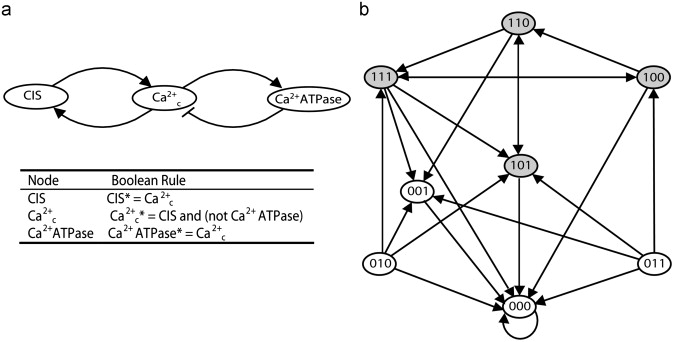
\includegraphics[width=0.9\linewidth]{gfx/red3nodos}
\caption[Modelo Booleano de 3 nodos]{Modelo Booleano de 3 nodos de \citeauthor{Reka3Nodos2010} \citep{Reka3Nodos2010}.\ Las flechas punteadas representan regulación positiva, mientras que las flechas planas representan regulación negativa.}\label{fig:red3reka}
\end{figure}

Las reglas lógicas para la red de $CIS$, $Ca^{2+}_c$ y $Ca^{2+}ATPase$ son

\begin{eqnarray}
   	CIS(t+1) & = & Ca^{2+}_c(t) \\ 
    Ca^{2+}_c(t+1) & = & CIS(t) \wedge \neg Ca^{2+}ATPase(t) \\ 
    Ca^{2+}ATPase(t+1) & = & Ca^{2+}_c(t)
\end{eqnarray}

Los símbolos $\land$, $\lor$ y $\neg$ representan las funciones lógicas Y (AND), O (OR) y Negación (NOT), respectivamente.

Por simplicidad, y debido a que el interés de trabajar con esta red es usar un modelo pequeño independientemente de las interpretaciones que se puedan hacer de la vía de señalización del ácido abscísico, denotemos a $CIS$, $Ca^{2+}_c$ y $Ca^{2+}ATPase$ como $\sigma_x$, $\sigma_y$ y $\sigma_z$, respectivamente. Las reglas lógicas quedan entonces como

\begin{eqnarray}
	\sigma_x(t+1) & = & \sigma_y(t) \\ 
    \sigma_y(t+1) & = & \sigma_x(t) \wedge \neg \sigma_z(t) \\ 
    \sigma_z(t+1) & = & \sigma_y(t)
\end{eqnarray}

El modelo de ecuaciones de Glass para la red de tres nodos queda dado por

\begin{eqnarray}\label{glass1_3nodos}
\frac{d\sigma_x}{dt} & = & \alpha_{\sigma_x} [F_{\sigma_x}(\widehat{\sigma_y(t)}) - \sigma_x(t)]
\end{eqnarray}
\begin{eqnarray}\label{glass2_3nodos}
\frac{d\sigma_y}{dt} & = & \alpha_{\sigma_y} [F_{\sigma_y}(\widehat{\sigma_x(t)}, \widehat{\sigma_z(t)}) - \sigma_y(t)]
\end{eqnarray}
\begin{eqnarray}\label{glass3_3nodos}
\frac{d\sigma_z}{dt} & = & \alpha_{\sigma_z} [F_{\sigma_z}(\widehat{\sigma_y(t)}) - \sigma_z(t)]
\end{eqnarray}
\\
donde

\begin{eqnarray}
	\widehat{\sigma_x}(t) = H(\sigma_x(t) - \theta_{\sigma_x}) \\
	\widehat{\sigma_y}(t) = H(\sigma_y(t) - \theta_{\sigma_y}) \\
	\widehat{\sigma_z}(t) = H(\sigma_z(t) - \theta_{\sigma_z})
\end{eqnarray}
\\
corresponden a los valores discretizados de las variables continuas $\sigma_x$, $\sigma_y$ y $\sigma_z$ al tiempo $t$, respectivamente, $H$ es la función de Heavyside y los $\theta_{\sigma_i}$ son valores de umbral. Es necesario discretizar el valor de estas variables pues hay que recordar que $F_{\sigma_x}$, $F_{\sigma_y}$ y $F_{\sigma_z}$ son funciones cuyos argumentos son valores discretos.




%\begin{table}
%    \myfloatalign
%  \begin{tabularx}{\textwidth}{Xll} \toprule
%    \tableheadline{labitur bonorum pri no} & \tableheadline{que vista}
%    & \tableheadline{human} \\ \midrule
%    fastidii ea ius & germano &  demonstratea \\
%    suscipit instructior & titulo & personas \\
%    %postulant quo & westeuropee & sanctificatec \\
%    \midrule
%    quaestio philosophia & facto & demonstrated \\
%    %autem vulputate ex & parola & romanic \\
%    %usu mucius iisque & studio & sanctificatef \\
%    \bottomrule
%  \end{tabularx}
%  \caption[Autem usu id]{Autem usu id.}
%  \label{tab:moreexample}
%\end{table}
%
%Ei solet nemore consectetuer nam. Ad eam porro impetus, te choro omnes
%evertitur mel. Molestie conclusionemque vel at, no qui omittam
%expetenda efficiendi. Eu quo nobis offendit, verterem scriptorem ne
%vix.
%
%  
%\begin{lstlisting}[float,caption=A floating example]
%for i:=maxint to 0 do
%begin
%{ do nothing }
%end;
%\end{lstlisting}